% !TeX program = xelatex
% This must be in the first 5 lines to tell arXiv to use pdfLaTeX, which is strongly recommended.
%\pdfoutput=1
% In particular, the hyperref package requires pdfLaTeX in order to break URLs across lines.


\documentclass[11pt]{article}

% Remove the "review" option to generate the final version.
\usepackage{acl}

\usepackage{subfig}
% Standard package includes
\usepackage[english]{babel}
\usepackage{xcolor}
\usepackage{rotating}
\usepackage{multirow}
\usepackage{xspace}
\usepackage{latexsym}
\usepackage{graphicx}
\usepackage{hyperref}
\usepackage{array}
\usepackage{color, colortbl}
\usepackage[inline]{enumitem}
\usepackage[flushleft]{threeparttable}
% For proper rendering and hyphenation of words containing Latin characters (including in bib files)

%\usepackage{devanagari}
\usepackage{times}
\usepackage[T1]{fontenc}
\usepackage{polyglossia} % Automatically loads fontspec
\setmainlanguage{english}
\setmainfont{Times New Roman}
\setotherlanguages{hindi}
\setotherlanguages{arabic}
\newfontfamily\hindifont{Hind-Light.ttf}[Script=Devanagari] % \texthindi{}
\newfontfamily\arabicfont{Amiri-Regular.ttf}[Script=Arabic] % \textarabic{}

% This assumes your files are encoded as UTF8
\usepackage[utf8]{inputenc}

% This is not strictly necessary, and may be commented out,
% but it will improve the layout of the manuscript,
% and will typically save some space.
\usepackage{microtype}

\usepackage{multirow}
\usepackage{graphicx}
\usepackage{threeparttable}

\title{\textbf{Separating Hate Speech and Offensive Language Classes via Adversarial Debiasing}}

\author{\textbf{Shuzhou Yuan} \and
\textbf{Antonis Maronikolakis} \and
\textbf{Hinrich Schütze}
}

\date{\texttt{shuzhou.yuan@outlook.com} ~~~~~ \texttt{antmarakis@cis.lmu.de}}

\begin{document}
	\maketitle
	\begin{abstract}
		
		Research to tackle hate speech plaguing online media has made strides in providing solutions, analyzing bias and curating data. A challenging problem is ambiguity between hate speech and offensive language, causing low performance both overall and specifically for the hate speech class. It can be argued that misclassifying actual hate speech content as merely offensive can lead to further harm against targeted groups. In our work, we mitigate this potentially harmful phenomenon by proposing an adversarial debiasing method to separate the two classes. We show that our method works for English, Arabic German and Hindi, plus in a multilingual setting, improving performance over baselines.
		
	\end{abstract}
	
	\section{Introduction}\label{intro}
	
	Online hate speech has become a pernicious phenomenon of modern society and a lot of effort is being expended in tackling this challenge. While there has been plenty of work to develop automatic methods for hate speech detection \cite{schmidt2017survey}, this has proven to be a difficult challenge to tackle with impractically poor performance.
	
	In the NLP community, a prevailing convention is to frame this problem as a three-way classification: between \textit{hate speech}, \textit{offensive language} and \textit{neither} \cite{davidson,mulki-etal-2019-l,founta,mubarak-etal-2017-abusive,mathur-etal-2018-offend}. While this convention allows for the application of more traditional NLP pipelines, performance has been low \cite{mozafari2019bert,davidson} especially when it comes to generalization to unseen data \cite{hate_speech_cross_dataset}, with even humans struggling to distinguish hate speech \cite{chatzakou2017mean,are_you_racist}.
	
	In our work we also adopt the wide-spread 3-class definition of hate speech, where \textit{hate speech} is defined as language used to express hatred towards a targeted group/individual based on protected attributes such as race or religion, \textit{offensive language} contains offensive terms but is not targeting any group in particular, while \textit{neither} is the case where none of the other two classes are present. As an example, in Table \ref{example} we present the tweets that are annotated as hate speech and offensive language respectively, from \citet{davidson}, alongside \texttt{DistilBERT} predictions.
	
	\begin{figure}[t!]
		\centering
		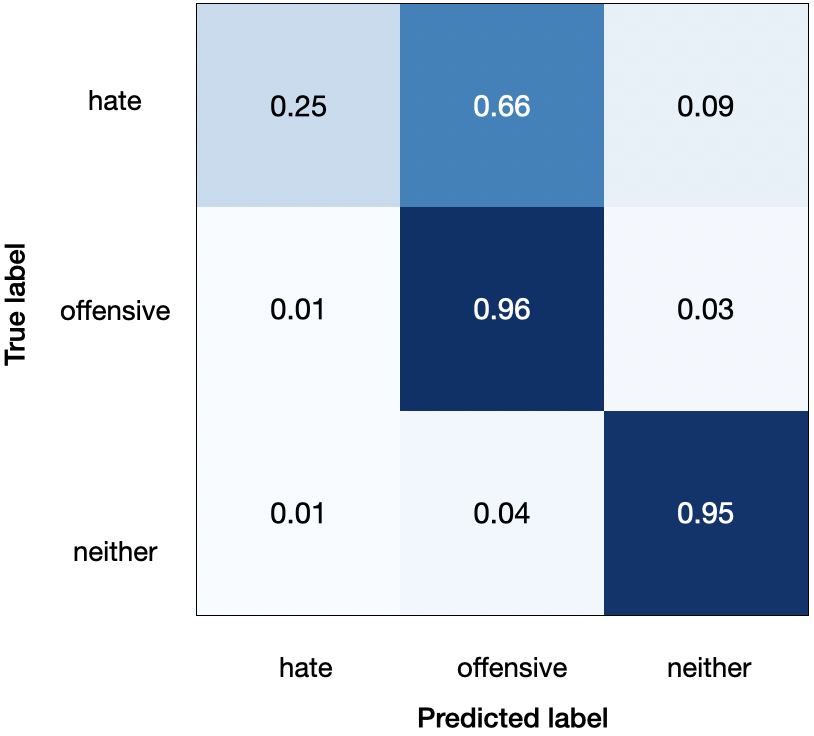
\includegraphics[scale=0.475]{BERT_classifier.png}
		\caption{Performance of \texttt{BERT} on \citet{davidson}. We see the confusion between hate speech and offensive language, with numerous False Negatives. We argue that these are very insidious mistakes that could lead to further harm against target groups. With our adversarial debiasing method, we can separate these two classes further and thus minimize this type of error as well as increase overall performance.}
		\label{pitch}
	\end{figure}
	
	An observation that can be made from the way classifiers operate is that oftentimes hate speech is misclassified as offensive language and vice-versa \cite{davidson,mozafari2019bert}. We showcase this in Figure \ref{pitch}. We argue that for hate speech detection models to be trustworthy, we need to work along two axes: increasing overall efficiency while keeping false negatives (i.e., hate speech marked as offensive language) to a minimum, and that we cannot have one if it comes at the expense of the other. Thus, models should be able to tackle both challenges simultaneously. If models have low accuracy, they will not find application in real-world settings, and if there is too much hate speech content slipping through the cracks, targeted communities will experience increased harm online.
	
	With that goal in mind, we propose a novel method to separate the two classes (\textit{hate speech} and \textit{offensive language}) via adapting adversarial debiasing methods to the problem at hand. This model stabilizes and improves classifier behavior and performance, increasing metrics across all classes, while at the same time keeping performance for hate speech content stable (or improving upon it). We thus strike a balance between performance overall and specifically for hate speech.
	
	We experiment with different architectures for the classifier (\texttt{BERT} \cite{devlin2019bert}, \texttt{DistilBERT} \cite{sanh2020distilbert}) and the adversary (\texttt{BERT}, \texttt{DistilBERT} and LSTMs \cite{lstm}). We perform hyperparameter tuning on English data before applying our findings on several languages (German, Arabic and Hindi) diverse in script, typography and grammar, as well as on a multilingual task setting using \texttt{mBERT}. To more objectively frame the benefit of our method, we compare against a battery of baselines, while we also perform error analysis to identify patterns where our method helps.
	
	In summary, our contributions\footnote{Code available at REMOVED\_FOR\_ANONYMITY} are: \begin{enumerate*}[label={\textbf{\roman{*})}}]
		\item Employing adversarial debiasing to separate hate speech and offensive language
		\item Showing that our method works in keeping false negatives to a minimum and increasing F1-scores on multiple English datasets
		\item Generalizing our findings to other languages, including a multilingual setting.
	\end{enumerate*}
	
	\begin{table}
		\centering
		\small
		\footnotesize
		\begin{tabular}{ccc}
			\hline\rule{0pt}{0.85\normalbaselineskip} \textbf{tweet} & \textbf{class} & \textbf{prediction} \\
			\hline\rule{0pt}{0.85\normalbaselineskip} bitch get off my twitter hoe  & offensive & offensive\\
			\hline\rule{0pt}{0.85\normalbaselineskip} You ain't gunna do shit\\spear chucker & hateful & offensive\\
			\hline\rule{0pt}{0.85\normalbaselineskip} LMFAO I HATE\\BLACK PEOPLE & hateful & hateful\\\hline
		\end{tabular}
		\caption{Labeled tweets (from \citet{davidson}) alongside model prediction.
			\label{example}}
	\end{table}
	
	
	\section{Related Work}
	
	For hate speech detection, supervised learning approaches are often used. \citet{schmidt2017survey} provide a comprehensive survey on the earlier research of hate speech detection. In more recent work, focus has been placed on various classification methods and curation of datasets \cite{davidson,wulczyn2017ex,zhang2018detecting,mozafari2019bert,qian-etal-2021-lifelong}. 
	
	In \citet{davidson}, the prevailing definition of the task as a three-way classification was formulated concretely. In their work, despite the high overall accuracy, over 30\% of hate speech was misclassified as offensive language, which saliently sheds light on this pervasive challenge in hate speech detection. This finding was corroborated more recently in \citet{mozafari2019bert}, where the state-of-the-art \texttt{BERT} model \cite{devlin2019bert} was applied on a hate speech detection task, with over 60\% of hate speech misclassified as offensive language. In the other direction, efforts have also been made to tackle false positives \cite{markov-daelemans-2021-improving}.
	
	Further, recent efforts in hate speech detection have increased language coverage from English to multiple languages around the globe, including Hindi \cite{mathur-etal-2018-offend}, Arabic \cite{mubarak-etal-2017-abusive}, Levantine \cite{mulki-etal-2019-l}, Indonesian \cite{ibrohim-budi-2019-multi}, Danish \cite{sigurbergsson-derczynski-2020-offensive} as well as more general multilingual data \cite{multi_hate_speech,hatespeech_crosslingual_embds,basile-etal-2019-semeval} and code-mixing \cite{bohra-etal-2018-dataset}.
	
	A similar methodology to adversarial debiasing was applied to recidivism prediction \cite{wadsworth2018achieving}. There, racial biases existing in criminal history datasets were mitigated through adversarial training. This method was also applied in hate speech research to minimize bias against AAE text \cite{adversarial_training_aae_hatespeech}. In this case, adversarial debiasing was employed to counteract the disproportionate labeling of AAE text as offensive or hate speech. These works have shown the potential of adversarial debiasing methods in training fairer models.
	
	
	\section{Data}
	
	 Since we wanted to evaluate the 3-class setting (\textit{hate speech}, \textit{offensive language} and \textit{neither}), we either used datasets that already utilized these classes or equivalent ones (for example, in \citet{founta} \textit{offensive language} is called \textit{abusive language}). Overall, we made use of seven datasets. A summary of each dataset is presented in Table \ref{data_summary}.
	
	\begin{table*}[ht!]
		\centering
		\small
		\scalebox{0.91}{
			\begin{tabular}{|c|c|c|c|c|}
				\hline
				Language & Dataset & Domain & Classes: size & Source  \\
				\hline
				\multirow{9}{*}{English} & \multirow{3}{*}{Davidson17} & \multirow{3}{*}{Twitter} & hate speech: 1431 &  \multirow{3}{*}{\citealt{davidson}} \\
				\cline{4-4}
				~& ~ & ~ &  offensive language: 19190 & ~ \\
				\cline{4-4}
				~ & ~ & ~ & neither: 4163 & ~ \\
				\cline{2-5}
				~ & \multirow{3}{*}{Founta18} & \multirow{3}{*}{Twitter} & hate speech: 4065 & \multirow{3}{*}{\citealt{founta}}\\
				\cline{4-4}
				~ & ~ & ~ &  abusive (OFF): 17150 & ~ \\
				\cline{4-4}
				~ & ~ & ~ & normal (NEI): 53851 & ~ \\
				\cline{2-5}
				~ & \multirow{3}{*}{HasocEn19} & \multirow{3}{*}{Twitter, Facebook} & hate speech: 1143 & \multirow{3}{*}{\citealt{mandl2019overview}}\\
				\cline{4-4}
				~ & ~ & ~ & offensive $\cup$ profanity (OFF): 1118 & ~ \\
				\cline{4-4}
				~ &  ~ & ~ & none (NEI): 3591 & ~ \\
				\hline
				\multirow{6}{*}{German} & \multirow{3}{*}{GermEval18} & \multirow{3}{*}{Twitter} & abuse (HAT): 1022 &  \multirow{3}{*}{\citealt{wiegand2018overview}} \\
				\cline{4-4}
				~& ~ & ~ & insult $\cup$ profanity (OFF): 19190 & ~ \\
				\cline{4-4}
				~ & ~ & ~ & Other(NEI): 3321 & ~ \\
				\cline{2-5}
				~ & \multirow{3}{*}{HasocDe19} & \multirow{3}{*}{Twitter, Facebook} & hate speech: 111 &  \multirow{3}{*}{\citealt{mandl2019overview}} \\
				\cline{4-4}
				~& ~ & ~ & offensive $\cup$ profanity (OFF): 296 & ~ \\
				\cline{4-4}
				~ & ~ & ~ & none(NEI): 3412 & ~ \\
				\hline
				\multirow{3}{*}{Arabic} & \multirow{3}{*}{L-HSAB19} & \multirow{3}{*}{Twitter} & hate speech: 417 &  \multirow{3}{*}{\citealt{mulki-etal-2019-l}} \\
				\cline{4-4}
				~& ~ & ~ & abusive (OFF): 1559 & ~ \\
				\cline{4-4}
				~ & ~ & ~ & normal (NEI): 3285 & ~ \\
				\hline
				\multirow{3}{*}{Hindi} & \multirow{3}{*}{HasocHin19} & \multirow{3}{*}{Twitter, Facebook} & hate speech: 556 &  \multirow{3}{*}{\citealt{mandl2019overview}} \\
				\cline{4-4}
				~& ~ & ~ & offensive $\cup$ profanity (OFF): 1913 & ~ \\
				\cline{4-4}
				~ & ~ & ~ & none (NEI): 2197 & ~ \\
				\hline
		\end{tabular}}
		\caption{Summary of the datasets used in our research. HAT: hate speech, OFF: offensive language, NEI: neither}
		\label{data_summary}
	\end{table*}
	
	
	\subsection{English}
	\textbf{Davidson17.} \citet{davidson} is a well-studied English hate speech dataset collected from Twitter. It contains 25K tweets that are annotated as hate speech, offensive (but not hate) speech, or neither hate speech nor offensive language. The definition of hate speech and offensive language is the same as in \S\ref{intro}. We utilize this dataset's development set for the early phase of experimentation to make design decisions, eg. selecting model architectures, hyperparameters, baselines, etc.
	
	\textbf{Founta18.} \citet{founta} contains 100K English samples collected from Twitter. The definition of hate speech is the usual definition (as described in \S\ref{intro}), while the \textit{abusive language} class is defined as any impolite content using profanity, which is equivalent to the definition of offensive language. Thus, we regard it as offensive language for our experiments.
	
	\textbf{HasocEn19.} \citet{mandl2019overview} is an English hate speech dataset of 6K samples from Twitter and Facebook. The samples were labeled into four categories: \textit{hate speech}, \textit{offensive language}, \textit{profanity}, and \textit{normal}. \textit{Offensive language} is defined as unacceptable language in the absence of insults and abuse. The \textit{profanity} class expands on this definition to include swear words. We merged the two classes, because both classes meet our definition.
	
	\subsection{German}
	
	\textbf{GermEval18.} \citet{wiegand2018overview} is a Twitter dataset containing 5K German tweets annotated as abuse, insult, profanity, and other/normal. The authors define the class \textit{abusive} as behaviour that promotes dehumanization towards a target societal group or individual. Since it is as same as the aforementioned definition of hate speech, we rename it as hate speech in our research. \textit{Profanity} is defined as text containing profane words and the class \textit{insult} expresses a clear intention to insult or offend somebody. The two categories are merged into one class, \textit{offensive language}.
	
	\textbf{HasocDe19.} \citet{mandl2019overview} is a 4K German dataset collected from Twitter and Facebook. The classes of \textit{HasocDe19} are the same as \textit{HasocEn19}: hate speech, offensive language, profanity, and normal. Similarly, the class \textit{profanity} and \textit{offensive language} are merged in our work.
	
	\subsection{Arabic}
	
	\textbf{L-HSAB19.} \citet{mulki-etal-2019-l} contains 5K Arabic tweets. They were annotated as hate tweets, abusive tweets, and normal tweets. The definition of hate tweets is the same as our definition of hate speech in \S\ref{intro}. The abusive tweets are defined as including offensive, aggressive or insulting language, which is equivalent to our definition of offensive language. We rename the class \textit{abusive} as \textit{offensive language} in our work.
	
	\subsection{Hindi} 
	
	\textbf{HasocHin19.} \citet{mandl2019overview} is a dataset of 5k samples written in Hindi. This dataset also comes from the \textit{Hasoc} family of data, and therefore has the same classes: hate speech, offensive language, profanity and normal. As with the other two \textit{Hasoc} datasets, the classes \textit{offensive language} and \textit{profanity} are merged into \textit{offensive language}.
	
	
	\section{Adversarial Debiasing}
	
	In this section, we detail our adversarial debiasing scheme. In this setup two models are trained in conjunction: the classifier (predictor) and the adversary. The classifier is predicting the actual class of an example, while the adversary learns to predict a protected variable.
	
	For the classifier, we compare the performance of three different models. And for the adversary, we investigate three different architectures, loss functions and protected variables\footnote{In some papers it is called ``protected attribute/label".}. In a first step, the models are trained and evaluated with \textit{Davidson17}, \textit{Founta18} and \textit{HasocEn19} (the English datasets in our experiments).
	
	\subsection{Classifier}
	
	In the adversarial debiasing setting, the classifier is the component making predictions for the given task. The goal is to use the adversarial component to ``debias" the classifier in order to achieve a desired result. In our case, our goal is to separate the \textit{hate speech} from the \textit{offensive language} class. We hypothesize this is going to improve performance. Here we explored \texttt{BERT}, \texttt{DistilBERT} and LSTM models for the classifier.
	
	\begin{figure*}[htbp]%
		\subfloat[][LSTM]{{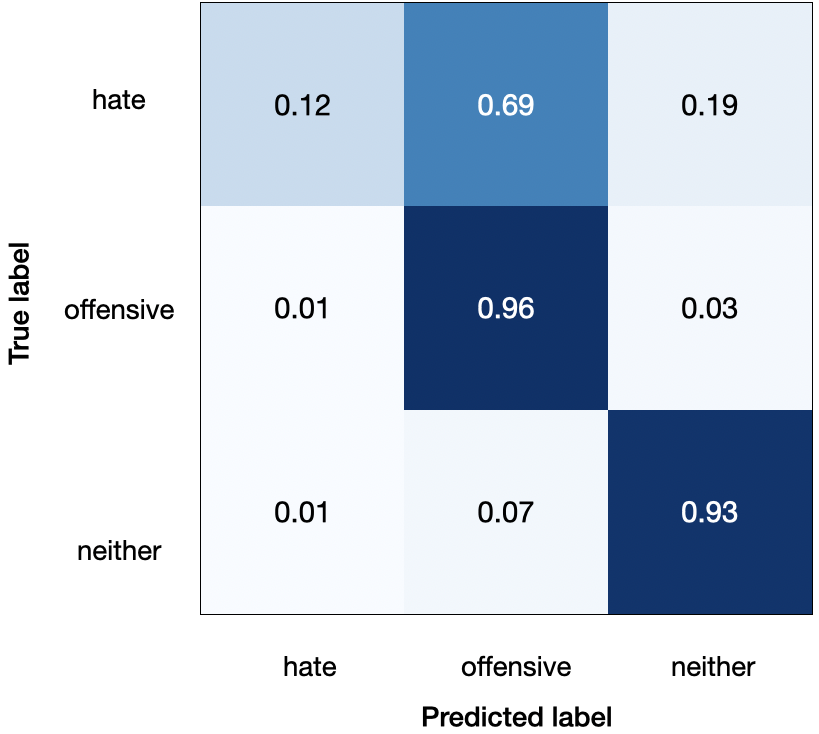
\includegraphics[width=4.7cm]{LSTM_classifier.png} }}%
		\qquad
		\subfloat[][DistilBERT]{{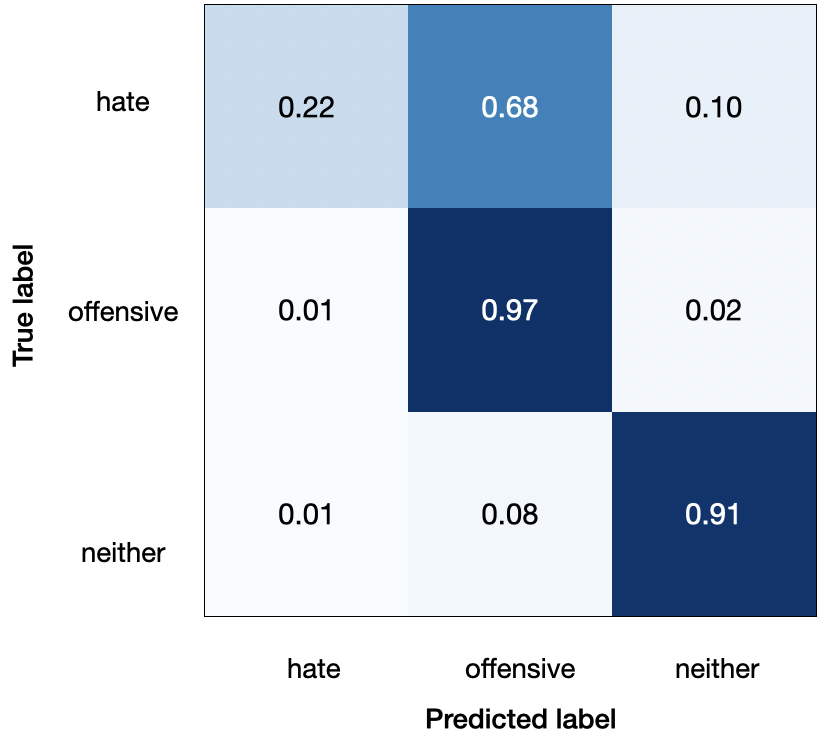
\includegraphics[width=4.7cm]{DistilBERT_classifier.png} }}%
		\qquad
		\subfloat[][BERT]{{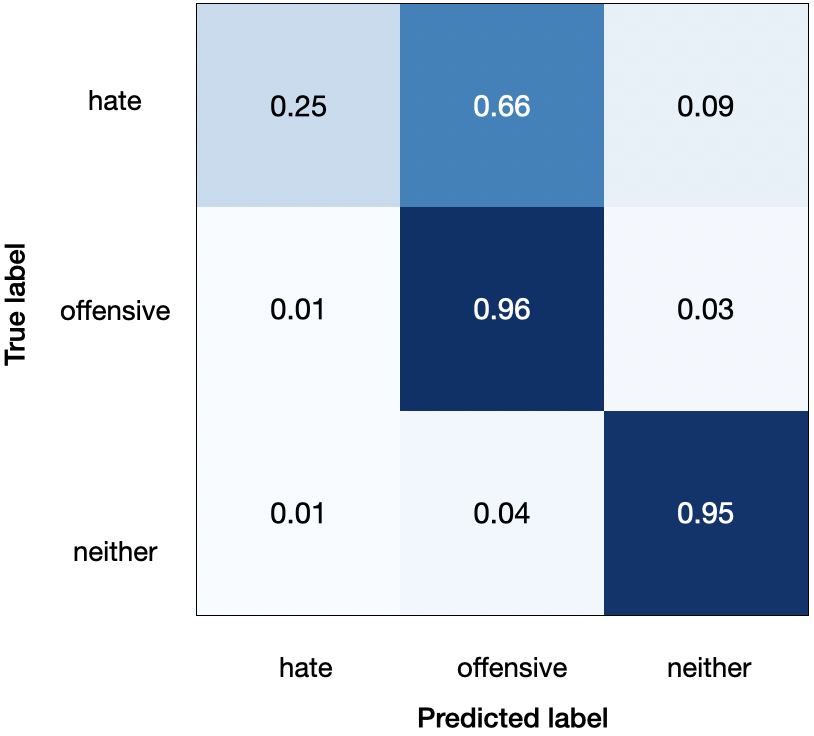
\includegraphics[width=4.7cm]{BERT_classifier.png} }}%
		\centering\caption{Confusion matrices for different classifier models}\label{classifier_confusion}
	\end{figure*}
	
	In our preliminary experiments (without adversarial debiasing), we found that LSTMs performed poorly in classifying hate speech. \texttt{BERT} and \texttt{DistilBERT} fared much better. All models, though, made a lot of false positive predictions, classifying hate speech as offensive language. Since \texttt{BERT} and \texttt{DistilBERT} had the highest true positive rate and both had similar performance, we chose to continue experimentation with \texttt{DistilBERT} to save on computational resources without a large performance drop. Confusion matrices for all three models are shown in Figure \ref{classifier_confusion}.
	
	\subsection{Adversary}
	
	The adversary in the setup is used to debias the classifier, learning to predict a particular attribute given the representations learned by the classifier. Then, via joint updating of weights, the classifier learns to generate representations that are not useful to the adversary, i.e., the goal is for the adversary to be unable to complete its task. We experiment with various protected variables, loss functions and architectures.
	
	\subsubsection{Adversary Architecture}
	
	The classifier we used in our final experiments was \texttt{DistilBERT}. Given some textual input, \texttt{DistilBERT} computes its internal representation which is then given as input to the adversary to predict the corresponding target. We experimented with two architectures for the adversary: Feed Forward Neural Networks (FFNs) and LSTMs. Accuracy for both adversaries was on average similar, plateauing around 75\%. Since there is little difference in accuracy, we chose the FFN as our adversary since it requires fewer computational resources.
	
	\subsubsection{Protected variable and loss function}
	\label{adv_setups}
	
	While in other research with adversarial debiasing \cite{adversarial_training_aae_hatespeech,aae_bias_hatespeech,diverse_adversaries_debiasing} has focused on debiasing for a protected variable (for example African American English), we instead propose a novel objective. In our experiments the adversary learns to predict the offensiveness of a sample, either by separating it from hate speech or merging it (and thus separating \textit{hate speech} and \textit{offensive language} in the classifier).
	
	\textbf{Adversary predicts \textit{hate speech} $\cup$ \textit{offensive language} jointly (\texttt{Adversary$_{joint}$}).}\footnote{Even though this method did not work consistently, we mention it as a good starting point of discussion.} Here the adversary is trying to jointly predict the \textit{hate speech} and \textit{offensive language} classes. Thus, we merge the two classes for the adversary's task, by labeling both classes as \textit{offensive}. \textit{Neither} is relabeled as \textit{not-offensive}. In this case, the adversary learns to predict all hate speech and offensive language examples as one class from the representation of the classifier. Thus, since the goal is for the adversary to be unable to do so, the classifier learns how to \textit{separate} these two classes. The loss function is defined as
	$$loss_{total}=loss_{classifier}-\alpha*loss_{adversary}.$$
	
	The loss function is the same as in \citet{wadsworth2018achieving,adversarial_training_aae_hatespeech}, with $loss_{adversary}$ being the loss of the adversary for its task, $loss_{classifier}$ the loss of the classifier for the original task (hate speech vs. offensive language vs. neither) and $\alpha$ being a parameter to regulate the effect of $loss_{adversary}$. \citet{adversarial_training_aae_hatespeech} found that the value should be neither too large nor too small. Empirically, they set $\alpha$=0.05. After some hyperparameter tuning, we found that in this setup an $\alpha$ value of 0.05 was the best-performing.
	Under $loss_{total}$, the classifier minimizes its original loss while maximizing the adversary's loss. As a result, the classifier is encouraged to actively develop diverging representations for the two classes.
	
	\textbf{Adversary discriminates between hate speech and offensive language (\texttt{Adversary$_{sep}$}).} We also experiment with another adversarial setup: the adversary acts like ``support", actively aiding the classifier in separating hate speech from offensive language. This is accomplished by employing an adversary that learns to model the "offensiveness" property, by discriminating between the \textit{hate speech}/\textit{neither} classes and \textit{offensive language}. Since this method is aimed at directly helping the classifier, instead of subtracting this adversary loss, we \textit{add} it instead:
	$$loss_{total}=loss_{classifier}+\alpha*loss_{adversary}.$$
	
	For this setup, we set the $\alpha$ hyperparameter to 2. The value of $\alpha$ was tuned on the development set of \textit{Davidson17}, achieving the highest true positive rate for hate speech.
	
	This ``supportive" setup (discriminating between \textit{hate speech} $\cup$ \textit{neither} and \textit{offensive}) was the best performing, so for the majority of our experiments we are using \texttt{Adversary$_{sep}$}.
	
	\textbf{Adversary predicts whether text contains swear words (\texttt{Adversary$_{swear}$}).}\footnote{This can only be applied in settings where swearword dictionaries are available, in our case we only applied it on the English datasets.} We also evaluated an adversary that predicts whether swear words are present in the text or not. We measured the proportion of \textit{hate speech} and \textit{offensive language} examples that contain a word from a dictionary of swear words\footnote{\url{https://www.cs.cmu.edu/~biglou/resources/bad-words.txt}} and found that in both classes more than 90\% of examples contain at least one swear word. A lot of hate speech is labeled by annotators as such because of the presence of swear words in the text even when that should not be an indicator of hatefulness \cite{aae_bias_hatespeech}.
	
	So, in this instance we train the adversary to predict whether swear words are present in text and then subtract this loss from the classifier's loss function. This forces the classifier to base its decisions on features other than the presence of swear words. The loss function is then
	$$loss_{total}=loss_{classifier}-\alpha*loss_{adversary}.$$
	
	
	
	\subsection{Class Rebalancing}
	
	One thing to note is that data is heavily imbalanced against hate speech across all datasets (Table \ref{data_summary}). For example, the number of offensive samples in \textit{Davidson17} is 15 times higher than the number of hate speech samples. Before our adversarial debiasing experiments, we perform a study on the effect of imbalance on the training set of \textit{Davidson17}. To compare against the original training set (denoted with \textit{original dataset}), we sampled equally-sized sets from each class. Henceforth, we call this new, balanced dataset \textit{uniform dataset}. Note that the development and testing sets remained unchanged for fair comparison: only the training sets were rebalanced. In Table \ref{Davidson_comparison} we see that the improvement of the true positive rate of hate speech is significant, from 22.0\% to 81.8\%. Although the overall accuracy drops by 16\%, we believe this model would be more applicable in a real world scenario. If we build hate speech detection models, we should be aiming for acceptable accuracy for the problematic class. Since we see that the uniform training set helps the model achieve acceptable performance for hate speech, we continue further experimentation using the uniform dataset.
	
	\begin{table}[h]
		\centering
		\small
		\begin{tabular}{|c|c|c|c|}
			\hline Data & Best TPH & Accuracy \\ \hline
			Original dataset &  22.0\% & 91.2\% \\\hline
			Uniform dataset  & 81.8\% & 75.2\% \\\hline
		\end{tabular}
		\caption{Comparison of original and uniform dataset with \textit{Davidson17}, evaluated on the same test set\label{Davidson_comparison}}
	\end{table}
	
	
	\section{Experimental Setup}
	
	For each dataset, we either use the provided training, development and testing set splits, or we sample them at 80:10:10 rates randomly. Then, we further downsample (to the number of examples in the smallest class according to each dataset) the training set classes to generate a uniform training set.
	
	For \textit{HasocEn19}, \textit{HasocDe19}, \textit{HasocHin19} and \textit{GermEval18}, the dataset was already split in training and test sets. The original rates are presented in Table \ref{original_rate}. In these cases, we keep the test set invariant and take 10\% samples from the training set to form our development set.
	
	\begin{table}[h]
		\centering
		\small
		\begin{tabular}{|c|c|}
			\hline Dataset & training:test \\ \hline
			\textit{HasocEn19} &  84:16 \\\hline
			\textit{HasocDe19}  & 82:18 \\\hline
			\textit{HasocHin19}  & 78:22 \\\hline
			\textit{GermEval18}  & 59:41 \\\hline
		\end{tabular}
		\caption{Original split distributions\label{original_rate}}
	\end{table}
	
	\begin{table*}[t!]
		\centering
		\small
		\begin{tabular}{|c|c|c|c|c|c|c|}
			\hline \multirow{2}{*}{~}  & \multicolumn{2}{c|}{Hate} & \multicolumn{2}{c|}{Offensive} & \multicolumn{2}{c|}{Neither}\\\cline{2-7}
			~ & total & \% & total & \% & total & \% \\\hline
			training set & 8,042 & 7.3\% & 42,037 & 38.0\% & 60,604 & 54.8\%  \\\hline
			dev set & 946 & 7.1\% & 5,204 & 38.3\% & 7,446 & 54.8\% \\\hline
			test set & 1,835 & 9.9\% & 5,925 & 32\% & 10,754 & 58.1\% \\\hline
			uniform training set & 8,042 & 33.3\% & 8,042 & 33.3\% & 8,042 & 33.3\% \\\hline
		\end{tabular}
		\caption{Class distribution in the training, development and testing sets of the multilingual dataset\label{multi_distribution}}
	\end{table*}
	
	For each experiment, we train for five epochs and keep the best-performing model across the epochs as evaluated on the development set. Then, we compute this model's performance on the held-out test set. We repeat this process three times and average the results.
	
	\textbf{Adversarial debiasing setup.} The main setup we examine is \texttt{Adversary$_{sep}$} where the adversary actively supports the classifier in separating the \textit{hate speech} from the \textit{offensive language} class, as defined in Section \ref{adv_setups}.
	
	\textbf{Multilingual dataset.} To obtain a multilingual hate speech dataset, we combine all the datasets in Table \ref{data_summary} together. This new multilingual hate speech dataset contains 110k samples with the distribution of the three classes presented in Table \ref{multi_distribution}.
	
	\textbf{Baselines.} To evaluate the benefits of our method, we compare against vanilla finetuning with \texttt{DistilBERT} on each hate speech dataset as well as a simple class weighting baseline. We experimented with different weights and found that the best performing one (on the \textit{Davidson17} dataset which served as an overall development set for design decisions) was $[1, 0.5, 1]$\footnote{[hate speech, offensive language, neither]}. That is, we halve the weight of the \textit{offensive} class.
	
	
	\section{Results}
	
	Results are summarized in Table \ref{all_result}. All the experiments are conducted on the uniform dataset, since the goal is to achieve an acceptable true positive rate (\textbf{TPH}: \textbf{T}rue \textbf{P}ositive rate for \textbf{H}ate speech) and this is a more solid starting point than the original distributions. We provide both macro and weighted F1 to show a more complete picture. Since our dataset is imbalanced, we focus on macro F1 for a more representative picture.
	
	For \textit{Davidson17} and \textit{Founta18}, our method does not provide positive findings. In \textit{Davidson17} both TPH and overall performance are lower, while in \textit{Founta18}, adversarial debiasing does provide a performance boost, but it comes at the expense of TPH. For these two datasets, \texttt{Adversary$_{swear}$} was applied as well, improving the TPH for \textit{Davidson17} but not for \textit{Founta18}.
	
	Results are better for the final English dataset, \textit{HasocEn19}. There, even though TPH drops substantially (10\%), overall performance increases by more than 20\%. Without an adversary, accuracy and F1-scores suffer, making for sub-par classifiers biased heavily towards hate speech. Instead, with our method, more separation is achieved and the model manages to separate the two contentious classes (\textit{hate speech} and \textit{offensive language}) with greater efficiency. Whereas before the classifier would not be practical due to low accuracy, with our method F1-scores and accuracy increase to acceptable levels.
	
	\textit{HasocDe19} follows the same pattern, with the vanilla model being unable to provide strong overall results, instead becoming biased towards hate speech and dropping the rest of the classes. With our method, better balance is struck and we see an improvement of 15\% over the vanilla model.
	
	In \textit{GermEval18}, we see stronger performance gains both for the TPH (+5.7\% over the non-adversary model) and overall (+2\% in F1-score). Even though the class-weighting baseline does score higher in TPH, we note a drop in F1-scores and accuracy.
	
	For \textit{HasocHin19}, we observe the same pattern as the other \textit{Hasoc} family of datasets, although to a lesser extent. In \textit{L-HSAB19}, we show that the simple class-weighting baselines is better than both the vanilla and adversary models.
	
	Finally, in the multilingual setting, we get mixed results. Compared to the vanilla model, adversarial debiasing offers a better TPH score with minimal drop in performance (while macro F1 increases by 2\% too). Against the baseline model, while the baseline has a higher TPH, in all the other metrics performance is worse.
	
	\begin{table*}[t!]
		\centering
		\small
		\begin{threeparttable}
			\begin{tabular}{|c|c|c|c|c|c|}
				\hline 
				Dataset & Experiment & Best TPH \% & Overall Accuracy\% & Macro F1 & Weighted F1 \\
				\hline
				\multirow{4}{*}{Davidson17} & Without adversary & 77.96 & \textbf{77.81} & \textbf{0.67} & \textbf{0.83} \\
				\cline{2-6}
				~ & Adversary$_{sep}$ & 76.88 & 76.88 & 0.66 & 0.82 \\
				\cline{2-6}
				~ & Adversary$_{swear}$ & \textbf{80.38} & 75.1 & 0.66 & 0.81 \\
				\cline{2-6}
				~ & Baseline & 78.77 & 72.64 & 0.64 & 0.79 \\
				\hline\hline
				\multirow{4}{*}{Founta18} & Without adversary & 74.37 & 78.22 & 0.67 & 0.83 \\
				\cline{2-6}
				~ & Adversary$_{sep}$ & 68.74 & \textbf{80.79} & \textbf{0.69} & \textbf{0.84} \\
				\cline{2-6}
				~ & Adversary$_{swear}$ & 73.24 & 77.82 & 0.67 & 0.82 \\
				\cline{2-6}
				~ & Baseline & \textbf{77.57} & 78.58 & 0.68 & 0.83 \\
				\hline\hline
				\multirow{4}{*}{HasocEn19} & Without adversary & 82.53 & 39.99 & 0.37 & 0.32 \\
				\cline{2-6}
				~ & Adversary$_{sep}$ & 72.58 & \textbf{47.53} & \textbf{0.47} & \textbf{0.54} \\
				\cline{2-6}
				~ & Baseline & \textbf{86.83} & 38.51 & 0.42 & 0.43 \\
				\hline\hline
				\multirow{4}{*}{GermEval18} & Without adversary & 50.41 & 63.66 & 0.53 & 0.65 \\
				\cline{2-6}
				~ & Adversary$_{sep}$ & 56.11 & \textbf{65.71} & \textbf{0.56} & \textbf{0.67} \\
				\cline{2-6}
				~ & Baseline & \textbf{63.86} & 64.45 & 0.53 & 0.65 \\
				\hline\hline
				\multirow{4}{*}{HasocDe19} & Without adversary & 75.00 & 31.11 & 0.25 & 0.39 \\
				\cline{2-6}
				~ & Adversary$_{sep}$ & 65.04 & \textbf{41.02} & \textbf{0.47} & \textbf{0.54} \\
				\cline{2-6}
				~ & Baseline & \textbf{92.68} & 38.67 & 0.42 & 0.43 \\
				\hline\hline
				\multirow{4}{*}{HasocHin19} & Without adversary & \textbf{79.90} & 58.67 & 0.56 & 0.63 \\
				\cline{2-6}
				~ & Adversary$_{sep}$ & 68.95 & 61.84 & \textbf{0.59} & \textbf{0.66} \\
				\cline{2-6}
				~ & Baseline & 73.08 & \textbf{62.92} & 0.58 & 0.66 \\
				\hline\hline
				\multirow{4}{*}{L-HSAB19} & Without adversary & 79.08 & 53.84 &0.48 & 0.58 \\
				\cline{2-6}
				~ & Adversary$_{sep}$ & 77.78 & 54.93 & 0.49 & 0.59  \\
				\cline{2-6}
				~ & Adversary$_{joint}$ & 81.04 & 54.64 & 0.50 & 0.58 \\
				\cline{2-6}
				~ & Baseline & \textbf{81.71} & \textbf{59.03} & \textbf{0.52} & \textbf{0.62} \\
				\hline\hline
				\multirow{4}{*}{Multilingual} & Without adversary & 77.04 & \textbf{72.37} & 0.63 & \textbf{0.76} \\
				\cline{2-6}
				~ & Adversary$_{sep}$ & 79.45 & 70.03 & \textbf{0.65} & 0.74 \\
				\cline{2-6}
				~ & Baseline & \textbf{81.85} & 68.41 & 0.63 & 0.73 \\
				\hline
			\end{tabular}
			% \begin{tablenotes}
				%     % \item[*]\textbf{TPH}: \textbf{T}rue \textbf{P}ositive rate for \textbf{H}ate speech
				%     %\item[1]Protected variable: offensive/not-offensive, hate as not-offensive
				%     %\item[2]Protected variable: contain/not contain bad words
				%     %\item[3]Protected variable: offensive/not-offensive, hate as offensive
				%   \end{tablenotes}
		\end{threeparttable}
		\caption{Summary of the results\label{all_result}}
	\end{table*}
	
	In synopsis, apart from \textit{L-HSAB19}, performance is better when using the adversarial debiasing method, either for the TPH or the overall F1-score metrics. For the multilingual dataset, performance of our method is mixed, improving upon the vanilla model on the TPH and upon the baseline model on the other metrics.
	
	All in all, our method manages to strike a better balance between TPH and overall performance and we thus believe these models are more applicable to a real-world scenario where both axes need to be taken into consideration.
	
	\section{Error Analysis}
	
	\begin{table*}[h!]
		\small
		\centering
		\begin{tabular}{|c|p{7.4cm}|c|c|c|}
			\hline Language & Text & True Label & Vanilla & Adversary\\ \hline
			en &  I can’t stress how much I hate these liberal Muslims that bend over backwards for these cunts and these Uncle Tom ass middle eastern / south Asian /Asian / african peoples who sell out like this & hate & offensive & hate\\\hline
			en & RT @user: This is one bad ass orangutan @emoji; @url & hate & offensive & hate\\\hline
			de & @user @user Glaubte Du echt, eine Frau mit befriedigendem Sexleben rennt durch die Welt und sieht überall böse Männer und sexuelle Gewalt? \textit{(@user @user Did you really believe that a woman with a satisfying sex life runs through the world and sees evil men and sexual violence everywhere?)}  & hate & offensive & hate\\\hline
			de & @user Genau. Die Froschfresser haben nichts gelernt! Ihr Untergang ist selbstverschuldet. \textit{(@user Exactly. The frog eaters haven't learned anything! Your downfall is self-inflicted.)} & hate & offensive & hate\\\hline
			hindi& {\hindifont झोंपड़ी के, कुछ दिन पहले तक तो तू उस आदतन 'बाइक चोर' तबरेज के लिये छाती पीट रहा था। हर चैनल पर रंडी रोना मचा रखा था। अब सेक्युलरिज्म का 'अखरोट' अपने पिछवाड़े से तोड़ने की कोशिश कर रहा है। आतंकी साला} \textit{(Of the hut, till a few days ago, you were habitually beating your chest for that `bike thief' Tabrez. Randi was crying on every channel. Now the `nut' of secularism is trying to break from its backyard. terrorist brother)} & offensive & hate & offensive\\\hline
			arabic& {\arabicfont  ما في اي شك بس الدروز كلاب و خونة} \textit{(True, there is no doubt, but the Druze are dogs and traitors)} & hate & offensive & hate\\\hline
		\end{tabular}
		\caption{Error analysis on predictions \texttt{DistilBERT} predictions versus actual predictions for the examined languages.\label{error_analysis}}
	\end{table*}
	
	We observe that a few samples of hate speech are misclassified as offensive language by the vanilla model without the adversary, but correctly predicted by the adversarial model. In Table \ref{error_analysis}, we collect 6 examples from different languages, which indicate the significant improvement of adversarial models.
	
	In English, we see that hateful speech was marked as merely offensive by the vanilla model, potentially because no slur was used, but only some offensive language (`c*nt', `ass' and `bad ass'). The model failed to take into account the context in which these words were used, or failed to pick up innocuous words used here as slurs (for example, `orangutan'). The adversarial model was able to make correct predictions, potentially because it is not putting as much weight on individual words, but the combinations between them.
	
	In German, the vanilla model's shortcomings are again centered around a lack of slurs. In both examples, there are no direct slurs so the model interprets it as offensive because of the overall negative sentiment (created through phrases such as `böse Männer', meaning `evil men' and `sexuelle Gewalt', meaning `sexual violence'). In one of the examples, the model misses that `Froschfresser' (meaning `frog eaters') is used as a slur. The adversarial model again shows an ability to expand from keyword-based predictions to a better understanding of context.
	
	In Hindi, while the example is merely offensive, the vanilla model has marked it as hateful, potentially because of the politically heavy `terrorist' term. The adversarial model has not put as much weight on the word and thus made a correct prediction. In Arabic, the vanilla model again misses that innocuous words are used as slurs (eg., `dogs'), marking the text as offensive instead of hateful.
	
	
	\section{Conclusion}
	
	In hate speech detection efforts, it can be observed that a lot of classifiers struggle with the \textit{hate speech} and \textit{offensive language} classes. A lot of models trained on current datasets misclassify hate speech as offensive language. We argue that this type of error is particularly insidious, since it can lead to targeted groups getting exposed to harmful content more often. Further, a lot of hate speech classifiers are impractical, either having a low true positive rate for hate speech or low performance overall.
	
	We propose a method to both increase the true positive rate for hate speech, but to also stabilize the classifiers in general. We base our method on the adversarial debiasing setup, where in our instance we are trying to support the classifier in separating the \textit{hate speech} and \textit{offensive language} classes.
	
	We evaluate our method on seven hate speech datasets spanning four languages, plus an additional multilingual dataset we create by combining the datasets at hand. Our method is at best performing just as well for all datasets except \textit{L-HSAB19}, while also outperforming baseline models in multiple occasions. Error analysis reveals that the debiased model is able to move past keyword-based predictions, taking into account the context as well. We find that both the true positive rate for hate speech is improved and overall performance is also higher, showcasing the stabilizing capabilities of our novel methodology on hate speech datasets.
	
	\section{Ethical Considerations}
	
	In our work we deal with hate speech, which could potentially cause harm (directly or indirectly) to vulnerable social groups. We do not support the views expressed in these hateful posts, we merely venture to analyze and provide solutions to mitigate this online phenomenon.
	
	Further, we could only examine a specific problem (neutral vs. offensive vs. hateful language) in specific languages. This is a non-exhaustive list and there is a lot we did not cover. Care should be taken to use these methods only in the examined languages since generalization may not be feasible (in fact, we show there are issues with our method in Arabic).
	
	
	
	
	
	
	% Entries for the entire Anthology, followed by custom entries
	% \clearpage
	% \newpage
	\bibliography{anthology}
	\bibliographystyle{acl_natbib}
	
	\appendix
	
	
	
\end{document}
